\documentclass[11pt]{article}

\usepackage[margin=1in]{geometry}
\usepackage{amsmath,amssymb,bm}
\usepackage{graphicx}
\usepackage{booktabs}
\usepackage{array}
\usepackage{float}
\usepackage{hyperref}

\graphicspath{{./}}

% Homework prompt, set off from the writeup that follows.
\newenvironment{question}{%
  \par\addvspace{0.8em}%
  \begin{quote}\small
  \noindent\textbf{Question.}\enspace\ignorespaces
}{%
  \end{quote}%
  \par\nopagebreak
  \noindent\textbf{Response.}\par\nopagebreak\smallskip
}

\title{Generative Models Homework Solutions}
\author{}
\date{}

\newcommand{\KL}{D_{\mathrm{KL}}}
\newcommand{\E}{\mathbb{E}}
\newcommand{\R}{\mathbb{R}}
\newcommand{\ind}{\mathbf{1}}

\begin{document}
\maketitle

\tableofcontents
\newpage

%%%%%%%%%%%%%%%%%%%%%%%%%%%%%%%%%%%%%%%%%%%%%%%%%%%%%%%%%%%%%%%%%%%%%%%%
\section{Problem 1: Kullback--Leibler Divergence (10 points)}
%%%%%%%%%%%%%%%%%%%%%%%%%%%%%%%%%%%%%%%%%%%%%%%%%%%%%%%%%%%%%%%%%%%%%%%%

\begin{question}
In class, we learned about KL divergence. Here, we like to understand why KL is not a true distance measure due to its asymmetric nature. Understanding the asymmetric nature of KL is critical in understanding the loss function in VAEs.
\begin{enumerate}
  \item[(a)] Generally \(\KL(P\|Q)\neq\KL(Q\|P)\). Give an example of univariate distributions \(P\) and \(Q\) where \(\KL(P\|Q)\neq\infty\) and \(\KL(Q\|P)=\infty\).
  \item[(b)] For a fixed target distribution \(P\), we call \(\KL(P\|Q)\) the forward KL and \(\KL(Q\|P)\) the reverse KL. Due to the asymmetric nature of KL, distributions \(Q\) that minimize \(\KL(P\|Q)\) can be different from those minimizing \(\KL(Q\|P)\). From the following plots, identify which of (A, B) corresponds to minimizing forward and reverse KL. Here, only the mean and standard deviation of \(Q\) are allowed to vary during the minimization. Give a brief reasoning.
  \begin{center}
    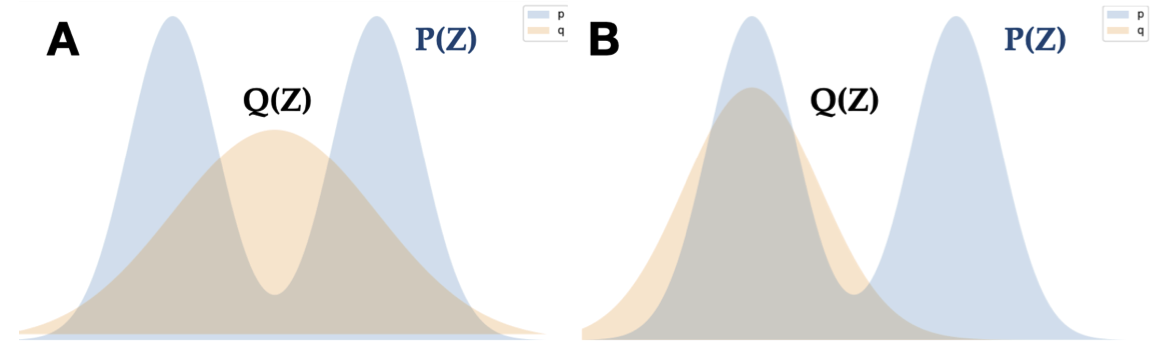
\includegraphics[width=\linewidth]{hw_kl_plots.png}
  \end{center}
  \item[(c)] What are the implications of this asymmetry in a VAE while maximizing the evidence lower bound
  \[
    \mathcal{L}(x;\theta,\phi)
    =\E_{q_\phi(z\mid x)}[\log p(x\mid z;\theta)]
    -\KL\bigl(q_\phi(z\mid x)\,\|\,p(z)\bigr)?
  \]
\end{enumerate}
\end{question}

KL is not a metric because it is asymmetric: in general
\(\KL(P\|Q)\neq\KL(Q\|P)\), and one direction can be infinite while the
other is finite. For densities \(p\) and \(q\),
\begin{equation}
  \KL(P\|Q)
  =\int p(x)\log\frac{p(x)}{q(x)}\,dx
  =\E_{x\sim P}\bigl[\log p(x)-\log q(x)\bigr].
\end{equation}
Two facts used below: \(\KL(P\|Q)\ge 0\) with equality iff \(P=Q\)
almost everywhere, and \(\KL(P\|Q)=\infty\) unless \(P\ll Q\). If there
is a set \(A\) with \(P(A)>0\) but \(Q(A)=0\), then
\(\log(p/q)=+\infty\) on a set of positive \(P\)-mass.

\subsection{Finite one way, infinite the other}

Take
\[
  p(x)=\ind_{[0,1]}(x),\qquad
  q(x)=\tfrac12\ind_{[0,2]}(x).
\]
The support of \(P\) sits inside the support of \(Q\), so
\[
  \KL(P\|Q)
  =\int_0^1 1\cdot\log\frac{1}{1/2}\,dx
  =\log 2<\infty.
\]
In the reverse direction,
\[
  \KL(Q\|P)
  =\int_0^1 \tfrac12\log\tfrac12\,dx
  +\int_1^2 \tfrac12\log\frac{1/2}{0}\,dx
  =\infty,
\]
because \(q>0=p\) on \((1,2]\). In general \(\KL(P\|Q)<\infty\) requires
\(\mathrm{supp}(P)\subseteq\mathrm{supp}(Q)\), while
\(\KL(Q\|P)=\infty\) as soon as that inclusion is strict. The same
pattern holds for \(P=\mathrm{Unif}[-a,a]\) and \(Q=\mathcal{N}(0,1)\).

\subsection{Forward KL vs.\ reverse KL}

Fix a (possibly multimodal) target \(P\) and restrict \(Q\) to a
unimodal family \(Q_{\mu,\sigma}=\mathcal{N}(\mu,\sigma^2)\). The two
objectives are expectations under \emph{different} measures:
\begin{align}
  \KL(P\|Q)
  &=\underbrace{\E_P[\log p]}_{\text{const in \(Q\)}
  }-\E_P[\log q],\\
  \KL(Q\|P)
  &=\E_Q[\log q]-\E_Q[\log p].
\end{align}

\paragraph{Forward KL \(\KL(P\|Q)\) is mode-covering.}
Minimizing it is equivalent to maximizing \(\E_P[\log q]\). Wherever
\(p(x)>0\) but \(q(x)\to 0\),
\[
  p(x)\log\frac{p(x)}{q(x)}\longrightarrow +\infty.
\]
Any hole of \(Q\) inside the support of \(P\) is infinitely expensive,
so the fitted \(Q\) must cover every mode of \(P\). With only mean and
variance free, that produces a wide, overdispersed Gaussian spanning
both peaks (plot~A).

\paragraph{Reverse KL \(\KL(Q\|P)\) is mode-seeking.}
The expectation is now under \(Q\). Mass of \(q\) in a valley where
\(p\approx 0\) costs \(+\infty\), so the optimizer zeros out \(q\)
wherever \(p\) is tiny. A unimodal \(Q\) therefore locks onto one mode
and shrinks \(\sigma\) to fit that peak (plot~B). Equivalently
\[
  \KL(Q\|P)=-H(Q)-\E_Q[\log p]:
\]
the entropy term favours a peaked \(Q\), and \(\E_Q[\log p]\) is large
only where \(p\) is large.

\begin{center}
\begin{tabular}{@{}lll@{}}
  \toprule
  & Forward \(\KL(P\|Q)\) & Reverse \(\KL(Q\|P)\) \\
  \midrule
  Expectation under & \(P\) (target) & \(Q\) (approximation) \\
  Infinite penalty & \(q=0\) where \(p>0\) & \(q>0\) where \(p=0\) \\
  Nickname & zero-avoiding / mode-covering & zero-forcing / mode-seeking \\
  Fitted Gaussian & wide, both peaks (A) & narrow, one peak (B) \\
  Variance bias & overestimates & underestimates \\
  \bottomrule
\end{tabular}
\end{center}

\subsection{Implications for the VAE ELBO}

The marginal likelihood of an observation \(x\) is
\[
  \log p_\theta(x)
  =\log\int q_\phi(z\mid x)\,\frac{p_\theta(x,z)}{q_\phi(z\mid x)}\,dz.
\]
Jensen's inequality yields the ELBO
\begin{equation}
  \mathcal{L}(x;\theta,\phi)
  =\E_{q_\phi(z\mid x)}\bigl[\log p_\theta(x\mid z)\bigr]
  -\KL\bigl(q_\phi(z\mid x)\,\|\,p(z)\bigr),
\end{equation}
with exact gap
\begin{equation}
  \log p_\theta(x)-\mathcal{L}(x;\theta,\phi)
  =\KL\bigl(q_\phi(z\mid x)\,\|\,p_\theta(z\mid x)\bigr).
\end{equation}
Maximizing \(\mathcal{L}\) over \(\phi\) is therefore exactly minimizing
the \emph{reverse} KL of the encoder against the true posterior. A
typical encoder \(q_\phi(z\mid x)=\mathcal{N}(\mu_\phi(x),\mathrm{diag}\,\sigma_\phi^2(x))\)
then inherits the geometry of plot~B:
\begin{enumerate}
  \item \textbf{Mode-seeking.} If \(p_\theta(z\mid x)\) is multimodal,
    \(q\) collapses onto one mode rather than covering all of them.
  \item \textbf{Underdispersed latents.} Because the gap is the reverse
    KL to the true posterior, \(q\) is pushed toward \(0\) wherever
    \(p_\theta(z\mid x)\) is small, so a Gaussian \(q\) tends to
    underestimate the posterior's spread. This is a separate quantity
    from the ELBO's own regularizer, the KL from \(q\) to the
    \emph{prior}, which for \(p(z)=\mathcal{N}(0,I)\) has the closed form
    \[
      \KL\bigl(q_\phi(z\mid x)\,\|\,p(z)\bigr)
      =\tfrac12\sum_i\bigl(\mu_i^2+\sigma_i^2-1-\log\sigma_i^2\bigr).
    \]
    The regularizer pulls each \(q_\phi(z\mid x)\) toward the prior, while
    the reconstruction term rewards a small \(\sigma\) around one good
    \(z\); the compromise is a tight blob per data point.
  \item \textbf{Posterior collapse.} If the decoder is powerful,
    \(\log p_\theta(x\mid z)\) can be large for every \(z\), and
    \(\mathcal{L}\) is then maximized by \(q_\phi(z\mid x)=p(z)\),
    independent of \(x\).
\end{enumerate}
The reconstruction term
\(\E_{q_\phi(z\mid x)}[\log p_\theta(x\mid z)]\) is also an expectation
under \(q\), so regions of latent space that \(q\) never visits do not
contribute. The decoder is trained only on the mode the encoder
selected.

%%%%%%%%%%%%%%%%%%%%%%%%%%%%%%%%%%%%%%%%%%%%%%%%%%%%%%%%%%%%%%%%%%%%%%%%
\section{Problem 2: EM for a Mixture of Bernoullis (20 points)}
%%%%%%%%%%%%%%%%%%%%%%%%%%%%%%%%%%%%%%%%%%%%%%%%%%%%%%%%%%%%%%%%%%%%%%%%

\begin{question}
You will derive an expectation-maximization (EM) algorithm to cluster black-and-white images. The inputs \(x^{(i)}\) can be thought of as vectors of binary values corresponding to black and white pixel values, and the goal is to cluster the images into groups. You will use a mixture of the Bernoulli model to tackle this problem.
\begin{enumerate}
  \item[(a)] Mixture of Bernoullis.
  \begin{enumerate}
    \item[(i)] Consider a vector of binary random variables \(x\in\{0,1\}^D\). Assume each variable \(x_d\) is drawn from a \(\mathrm{Bernoulli}(p_d)\) distribution, so \(P(x_d=1)=p_d\). Let \(p\in(0,1)^D\) be the resulting vector of Bernoulli parameters. Write an expression for \(P(x\mid p)\).
    \item[(ii)] Now suppose we have a mixture of \(K\) Bernoulli distributions: each vector \(x^{(i)}\) is drawn from some vector of Bernoulli random variables with parameters \(p^{(k)}\); we will call this \(\mathrm{Bernoulli}(p^{(k)})\). Let \(\{p^{(1)},\ldots,p^{(K)}\}=\mathbf{p}\). Assume a distribution \(\pi(k)\) over the selection of which set of Bernoulli parameters \(p^{(k)}\) is chosen. Write an expression for \(P(x^{(i)}\mid\mathbf{p},\pi)\).
    \item[(iii)] Finally, suppose we have inputs \(X=\{x^{(i)}\}_{i=1,\ldots,n}\). Using the above, write an expression for the log likelihood of the data \(X\), \(\log P(X\mid\pi,\mathbf{p})\).
  \end{enumerate}
  \item[(b)] Expectation step.
  \begin{enumerate}
    \item[(i)] Now we introduce the latent variables for the EM algorithm. Let \(z^{(i)}\in\{0,1\}^K\) be an indicator vector, such that \(z^{(i)}_k=1\) if \(x^{(i)}\) was drawn from a \(\mathrm{Bernoulli}(p^{(k)})\), and \(0\) otherwise. Let \(Z=\{z^{(i)}\}_{i=1,\ldots,n}\). What is \(P(z^{(i)}\mid\pi)\)? What is \(P(x^{(i)}\mid z^{(i)},\mathbf{p},\pi)\)?
    \item[(ii)] Using the above two quantities, derive the likelihood of the data and the latent variables, \(P(Z,X\mid\pi,\mathbf{p})\).
    \item[(iii)] Let \(\eta(z^{(i)}_k)=\E[z^{(i)}_k\mid x^{(i)},\pi,\mathbf{p}]\). Show that
    \[
      \eta(z^{(i)}_k)
      =\frac{
        \pi_k\prod_{d=1}^D
        (p^{(k)}_d)^{x^{(i)}_d}(1-p^{(k)}_d)^{1-x^{(i)}_d}
      }{
        \sum_j\pi_j\prod_{d=1}^D
        (p^{(j)}_d)^{x^{(i)}_d}(1-p^{(j)}_d)^{1-x^{(i)}_d}
      }.
    \]
    Let \(\hat{\mathbf{p}},\hat\pi\) be the new parameters that we would like to maximize, so \(\mathbf{p},\pi\) are from the previous iteration. Use this to derive the following final expression for the E step:
    \begin{align*}
      &\E\bigl[\log P(Z,X\mid\hat{\mathbf{p}},\hat\pi)\mid X,\mathbf{p},\pi\bigr]\\
      &\quad=
      \sum_{i=1}^N\sum_{k=1}^K
      \eta(z^{(i)}_k)
      \Biggl[
        \log\hat\pi_k
        +\sum_{d=1}^D
        \Bigl(
          x^{(i)}_d\log\hat p^{(k)}_d
          +(1-x^{(i)}_d)\log(1-\hat p^{(k)}_d)
        \Bigr)
      \Biggr].
    \end{align*}
  \end{enumerate}
  \item[(c)] Maximization step.
  \begin{enumerate}
    \item[(i)] We need to maximize the above expression with respect to \(\hat\pi,\hat{\mathbf{p}}\). First, show that the value of \(\hat p\) that maximizes the E step is
    \[
      \hat p^{(k)}
      =\frac{\sum_{i=1}^N\eta(z^{(i)}_k)\,x^{(i)}}{N_k},
      \qquad
      N_k=\sum_{i=1}^N\eta(z^{(i)}_k).
    \]
    \item[(ii)] Show that the value of \(\hat\pi\) that maximizes the E step is
    \[
      \hat\pi_k=\frac{N_k}{\sum_{k'}N_{k'}}.
    \]
    The exponential families notation may be useful. Alternatively, you can use Lagrange multipliers.
  \end{enumerate}
\end{enumerate}
\end{question}

\subsection{Mixture of Bernoullis}

Throughout the response, \(N\) denotes the number of images (the
question uses both \(n\) and \(N\) for it).

\paragraph{(i)}
Assume the coordinates of \(x\in\{0,1\}^D\) are independent given
\(p\in(0,1)^D\). Then
\begin{equation}
  P(x\mid p)
  =\prod_{d=1}^D p_d^{x_d}(1-p_d)^{1-x_d}.
\end{equation}

\paragraph{(ii)}
A cluster \(k\in\{1,\ldots,K\}\) is drawn from \(\pi\), then
\(x^{(i)}\) is generated from Bernoulli\((p^{(k)})\):
\begin{equation}
  P(x^{(i)}\mid \mathbf{p},\pi)
  =\sum_{k=1}^K \pi_k
  \prod_{d=1}^D
  \bigl(p_d^{(k)}\bigr)^{x_d^{(i)}}
  \bigl(1-p_d^{(k)}\bigr)^{1-x_d^{(i)}}.
\end{equation}

\paragraph{(iii)}
With i.i.d.\ observations \(X=\{x^{(i)}\}_{i=1}^N\),
\begin{equation}
  \log P(X\mid\pi,\mathbf{p})
  =\sum_{i=1}^N\log\Biggl(
    \sum_{k=1}^K \pi_k
    \prod_{d=1}^D
    \bigl(p_d^{(k)}\bigr)^{x_d^{(i)}}
    \bigl(1-p_d^{(k)}\bigr)^{1-x_d^{(i)}}
  \Biggr).
\end{equation}
The inner sum is why a direct MLE is inconvenient: the missing cluster
identity couples the parameters.

\subsection{Expectation step}

\paragraph{(i)}
Let \(z^{(i)}\in\{0,1\}^K\) be one-hot, with \(z_k^{(i)}=1\) iff image
\(i\) came from component \(k\). Then \(z^{(i)}\sim\mathrm{Categorical}(\pi)\),
\begin{equation}
  P(z^{(i)}\mid\pi)
  =\prod_{k=1}^K \pi_k^{z_k^{(i)}},
\end{equation}
and given \(z^{(i)}\) the mixture index is known, so \(\pi\) drops out:
\begin{equation}
  P(x^{(i)}\mid z^{(i)},\mathbf{p})
  =\prod_{k=1}^K
  \Biggl[
    \prod_{d=1}^D
    \bigl(p_d^{(k)}\bigr)^{x_d^{(i)}}
    \bigl(1-p_d^{(k)}\bigr)^{1-x_d^{(i)}}
  \Biggr]^{z_k^{(i)}}.
\end{equation}

\paragraph{(ii)}
Independence across images gives the complete-data likelihood
\begin{equation}
  P(Z,X\mid\pi,\mathbf{p})
  =\prod_{i=1}^N\prod_{k=1}^K
  \Biggl[
    \pi_k
    \prod_{d=1}^D
    \bigl(p_d^{(k)}\bigr)^{x_d^{(i)}}
    \bigl(1-p_d^{(k)}\bigr)^{1-x_d^{(i)}}
  \Biggr]^{z_k^{(i)}}.
\end{equation}
The complete-data log-likelihood is linear in the missing indicators:
\begin{equation}
  \log P(Z,X\mid\pi,\mathbf{p})
  =\sum_{i=1}^N\sum_{k=1}^K z_k^{(i)}
  \Biggl[
    \log\pi_k
    +\sum_{d=1}^D
    \Bigl(
      x_d^{(i)}\log p_d^{(k)}
      +(1-x_d^{(i)})\log(1-p_d^{(k)})
    \Bigr)
  \Biggr].
\end{equation}

\paragraph{(iii)}
The responsibility is the posterior of the indicator:
\begin{align}
  \eta(z_k^{(i)})
  &:=\E\bigl[z_k^{(i)}\mid x^{(i)},\pi,\mathbf{p}\bigr]
  =P\bigl(z_k^{(i)}=1\mid x^{(i)},\pi,\mathbf{p}\bigr) \nonumber\\
  &=\frac{
      \pi_k\prod_{d=1}^D
      \bigl(p_d^{(k)}\bigr)^{x_d^{(i)}}
      \bigl(1-p_d^{(k)}\bigr)^{1-x_d^{(i)}}
    }{
      \sum_{j=1}^K
      \pi_j\prod_{d=1}^D
      \bigl(p_d^{(j)}\bigr)^{x_d^{(i)}}
      \bigl(1-p_d^{(j)}\bigr)^{1-x_d^{(i)}}
    }.
\end{align}
Write \(\hat\pi,\hat{\mathbf{p}}\) for candidate parameters and
\(\pi,\mathbf{p}\) for the previous iterate. Conditioning on \(X\)
replaces every \(z_k^{(i)}\) by its posterior mean, which is the
\(Q\)-function
\begin{equation}
\begin{aligned}
  &\E\bigl[\log P(Z,X\mid\hat{\mathbf{p}},\hat\pi)\mid X,\mathbf{p},\pi\bigr]\\
  &\qquad=
  \sum_{i=1}^N\sum_{k=1}^K
  \eta(z_k^{(i)})
  \Biggl[
    \log\hat\pi_k
    +\sum_{d=1}^D
    \Bigl(
      x_d^{(i)}\log\hat p_d^{(k)}
      +(1-x_d^{(i)})\log(1-\hat p_d^{(k)})
    \Bigr)
  \Biggr].
\end{aligned}
\end{equation}
The \(\eta\) values are computed from the \emph{old} \((\pi,\mathbf{p})\)
and treated as constants in the M-step.

\subsection{Maximization step}

The \(Q\)-function separates in \(\hat\pi\) and the rows of
\(\hat{\mathbf{p}}\).

\paragraph{(i) Update for \(\hat p^{(k)}\).}
For coordinate \(d\) of cluster \(k\),
\[
  \sum_{i=1}^N \eta(z_k^{(i)})
  \Biggl(
    \frac{x_d^{(i)}}{\hat p_d^{(k)}}
    -\frac{1-x_d^{(i)}}{1-\hat p_d^{(k)}}
  \Biggr)
  =0
\]
simplifies to
\(\sum_i\eta(z_k^{(i)})\bigl(x_d^{(i)}-\hat p_d^{(k)}\bigr)=0\).
With \(N_k:=\sum_{i=1}^N\eta(z_k^{(i)})\),
\begin{equation}
  \hat p^{(k)}
  =\frac{\sum_{i=1}^N \eta(z_k^{(i)})\,x^{(i)}}{N_k}.
\end{equation}
This is a responsibility-weighted mean of the images. The second
derivative on \((0,1)\) is negative, so the critical point is a maximum.

\paragraph{(ii) Update for \(\hat\pi\).}
Maximize \(\sum_k N_k\log\hat\pi_k\) subject to
\(\sum_k\hat\pi_k=1\). The Lagrangian
\[
  \mathcal{L}(\hat\pi,\lambda)
  =\sum_{k=1}^K N_k\log\hat\pi_k
  +\lambda\Bigl(1-\sum_{k=1}^K\hat\pi_k\Bigr)
\]
gives \(N_k/\hat\pi_k=\lambda\). The simplex constraint forces
\(\lambda=\sum_{k'}N_{k'}\), hence
\begin{equation}
  \hat\pi_k
  =\frac{N_k}{\sum_{k'}N_{k'}}.
\end{equation}
(The same updates are the exponential-family moment match for
categorical \(\pi\) and Bernoulli \(p_d\).)

With Dirichlet smoothing \(\alpha_1=\alpha_2=10^{-8}\) as in the
implementation,
\begin{equation}
  \hat p^{(k)}
  =\frac{\sum_i\eta(z_k^{(i)})x^{(i)}+\alpha_1}{N_k+\alpha_1 D},\qquad
  \hat\pi_k
  =\frac{N_k+\alpha_2}{\sum_{k'}N_{k'}+\alpha_2 K}.
\end{equation}

%%%%%%%%%%%%%%%%%%%%%%%%%%%%%%%%%%%%%%%%%%%%%%%%%%%%%%%%%%%%%%%%%%%%%%%%
\section{Problem 3: Expectation--Maximization on MNIST (20 points)}
%%%%%%%%%%%%%%%%%%%%%%%%%%%%%%%%%%%%%%%%%%%%%%%%%%%%%%%%%%%%%%%%%%%%%%%%

\begin{question}
You will now cluster the images on the MNIST dataset by implementing the algorithm derived above. Each input is a binary number corresponding to black and white pixels and is a flattened version of the \(28\times 28\) pixel image. Conventions:
\begin{itemize}
  \item \(N=1000\) is the number of data points (sampled randomly from the full MNIST dataset), \(D\) is the dimension of each input, and \(K\) is the number of clusters.
  \item \(X_s\) is an \(N\times D\) matrix of the input data, where row \(i\) is the pixel data for picture \(i\).
  \item \(p\) is a \(K\times D\) matrix of Bernoulli parameters, where row \(k\) is the vector of parameters for the \(k\)th mixture of Bernoullis.
  \item \(\texttt{mix\_pi}\) is a \(K\times 1\) vector containing the distribution over the various mixtures.
  \item \(\texttt{eta}\) is an \(N\times K\) matrix containing the results of the E step, so \(\texttt{eta}[i,k]=\eta(z^{(i)}_k)\).
\end{itemize}
\begin{enumerate}
  \item[(a)] Implement the E step within \(\texttt{Estep}(X_s,p,\texttt{mix\_pi})\), saving the calculated values in the returned variable \(\texttt{eta}\).
  \item[(b)] Implement the M step within \(\texttt{Mstep}(X_s,\texttt{eta},\texttt{alpha1},\texttt{alpha2})\). Return the new values \(p\) and \(\texttt{mix\_pi}\) that maximize the E step. \(\texttt{alpha1}\) and \(\texttt{alpha2}\) are Dirichlet smoothing parameters.
  \item[(c)] Implement the full EM algorithm in \(\texttt{EM}(X_s,K,\texttt{iter})\) by alternating between the E and M steps for \(\texttt{iter}=20\) iterations. Return the final parameters \(p\) and \(\texttt{mix\_pi}\).
\end{enumerate}
Tips: use the log operator for numerical stability; avoid zeros in \(\pi\) and \(p\) with Dirichlet prior smoothing \(\alpha_1=\alpha_2=10^{-8}\),
\[
  \hat p^{(k)}
  =\frac{\sum_{i=1}^N\eta(z^{(i)}_k)x^{(i)}+\alpha_1}{N_k+\alpha_1 D},
  \qquad
  \hat\pi_k
  =\frac{N_k+\alpha_2}{\sum_{k'}N_{k'}+\alpha_2 K};
\]
initialize \(p\) by sampling from \(\mathrm{Uniform}(0,1)\) and normalizing each \(p^{(k)}\) to unit length, and set \(\pi_k=1/K\).
\begin{enumerate}
  \item[(d)] Run the EM algorithm and plot the resulting Bernoulli parameters \(p\). Reshape each row into a \(28\times 28\) matrix and print the resulting grayscale image. What do you see? Repeat the experiment for \(K=5\) and \(K=20\) and explain how the results differ.
  \item[(e)] Explain the process you would follow to generate new images using the parameters obtained through the above algorithm. Based on your observations from the three cases in the previous part, explain why (or why not) the generated images would be plausible samples from the ``original'' distribution.
\end{enumerate}
\end{question}

We implemented the algorithm above on \(N=1000\) randomly sampled,
binarized MNIST digits (\(D=784\)), with log-space softmax
responsibilities for numerical stability. Parameters \(p^{(k)}\) were
initialized from \(\mathrm{Unif}(0,1)\) and \(\ell_2\)-normalized;
\(\pi_k=1/K\). Each row of \(p\) is a mean image: pixel \(d\) is
\(P(\text{pixel }d=1\mid\text{cluster }k)\). The implementations of
\texttt{Estep}, \texttt{Mstep}, and \texttt{EM} for parts (a)--(c) are
listed in Appendix~\ref{app:em} (full script: \texttt{em\_mnist.py}).

\subsection{Fitted Bernoulli parameters}

\begin{figure}[H]
  \centering
  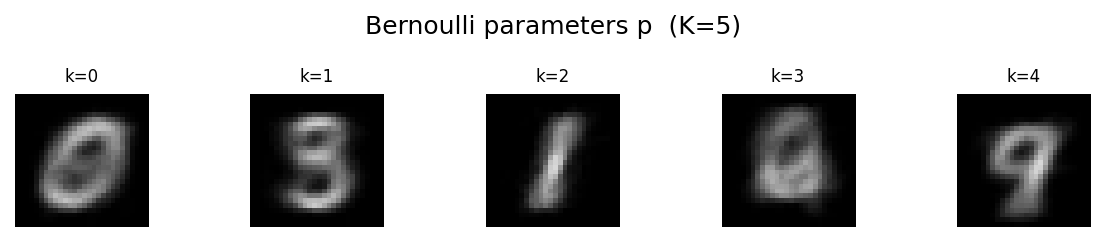
\includegraphics[width=\textwidth]{bernoulli_params_K5.png}
  \caption{\(K=5\): five coarse prototypes. Similar digits share a
    component, so the means are smeared (e.g.\ a \(3/5/8\)-like blob).}
\end{figure}

\begin{figure}[H]
  \centering
  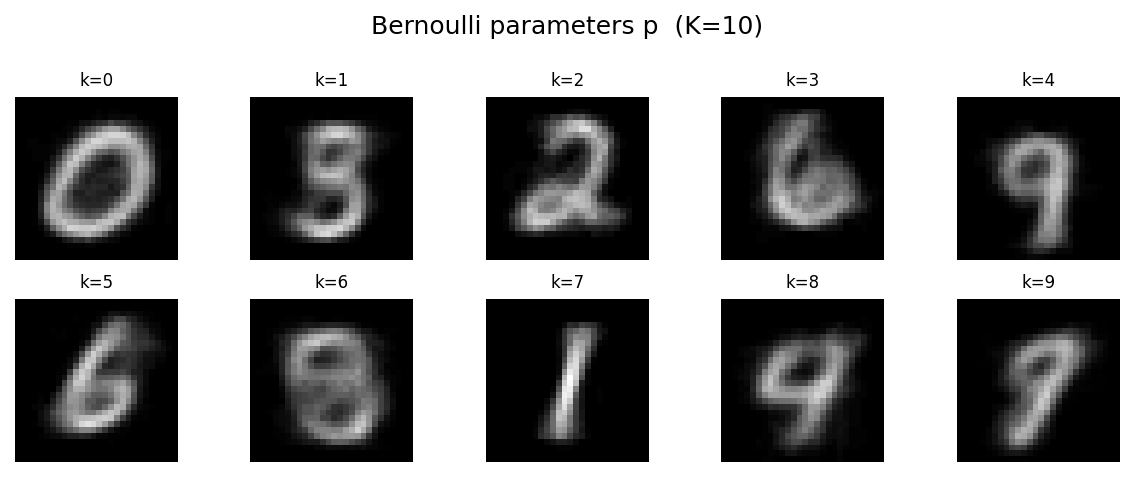
\includegraphics[width=0.9\textwidth]{bernoulli_params_K10.png}
  \caption{\(K=10\): more recognizable digits, but still not one cluster
    per class. EM clusters pixel patterns, not labels. Checking the
    hard assignments against the true labels: \(6\) gets two
    components (\(k=3\) and \(k=5\), 50 sixes each), while \(8\) is not
    the majority label of any component; its images split mainly
    between the \(3/5/8\) blend \(k=1\) and \(k=9\).}
\end{figure}

\begin{figure}[H]
  \centering
  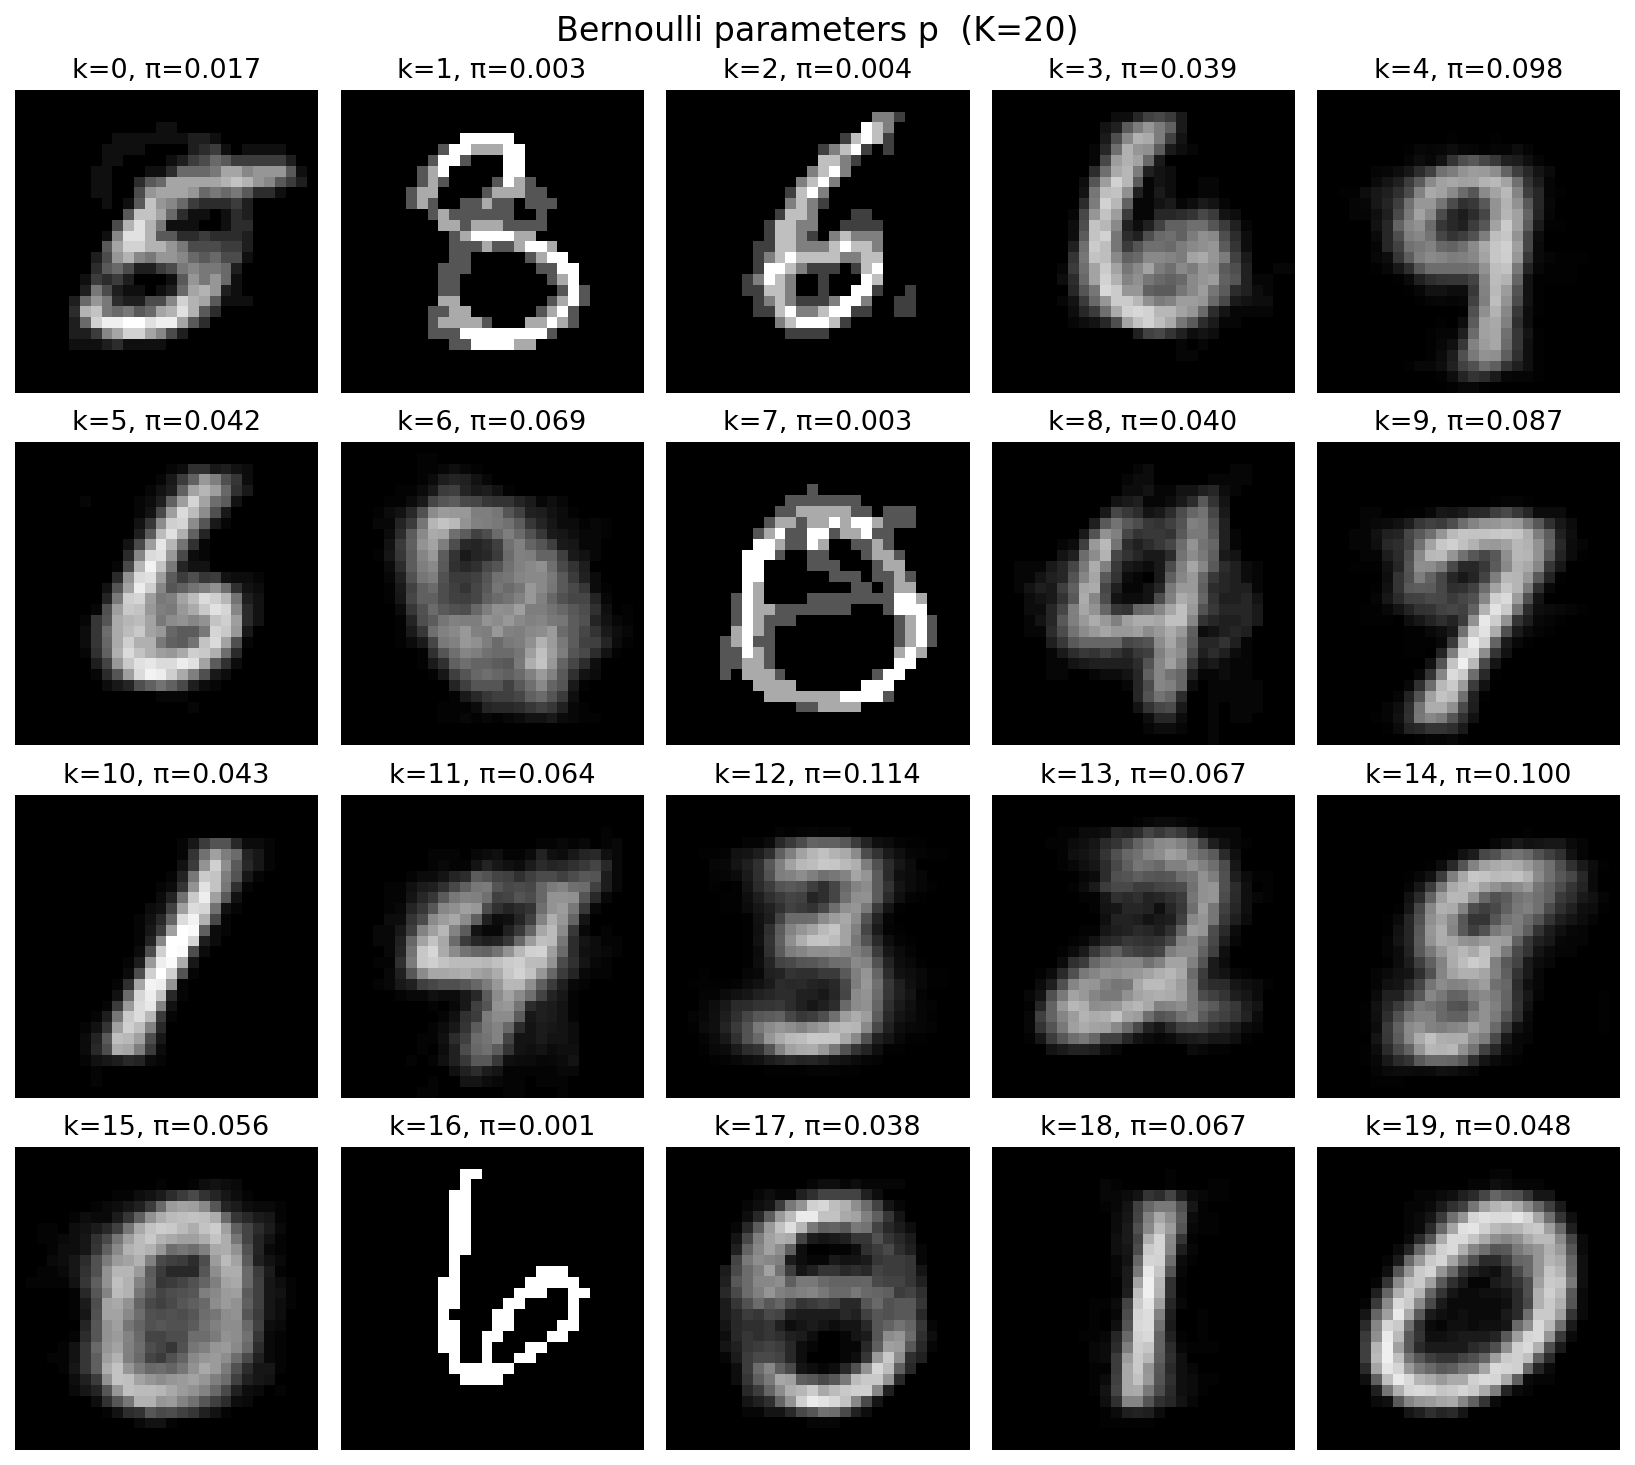
\includegraphics[width=0.78\textwidth]{bernoulli_params_K20.png}
  \caption{\(K=20\): sharper means and multiple writing styles of the
    same digit (panel titles show \(\pi_k\)). Four components
    (\(k=1,2,7,16\)) have \(\pi_k<0.005\) and capture at most four
    images each; \(k=16\) holds a single image.}
\end{figure}

The grayscale look is expected: \(p_d^{(k)}\in(0,1)\) is an expected
intensity, not a sampled binary image.

\subsection{Generating new images}

Ancestral sampling from the fitted mixture:
\begin{enumerate}
  \item Draw a cluster \(k\sim\mathrm{Categorical}(\pi)\).
  \item Independently draw each pixel \(x_d\sim\mathrm{Bernoulli}(p_d^{(k)})\).
\end{enumerate}
Those samples are \emph{not} plausible draws from the original digit
distribution. Conditional pixel independence is false for handwriting:
real digits are strokes, so neighbouring pixels are strongly dependent.
Independent Bernoullis produce salt-and-pepper snow around the mean
shape.

\begin{figure}[H]
  \centering
  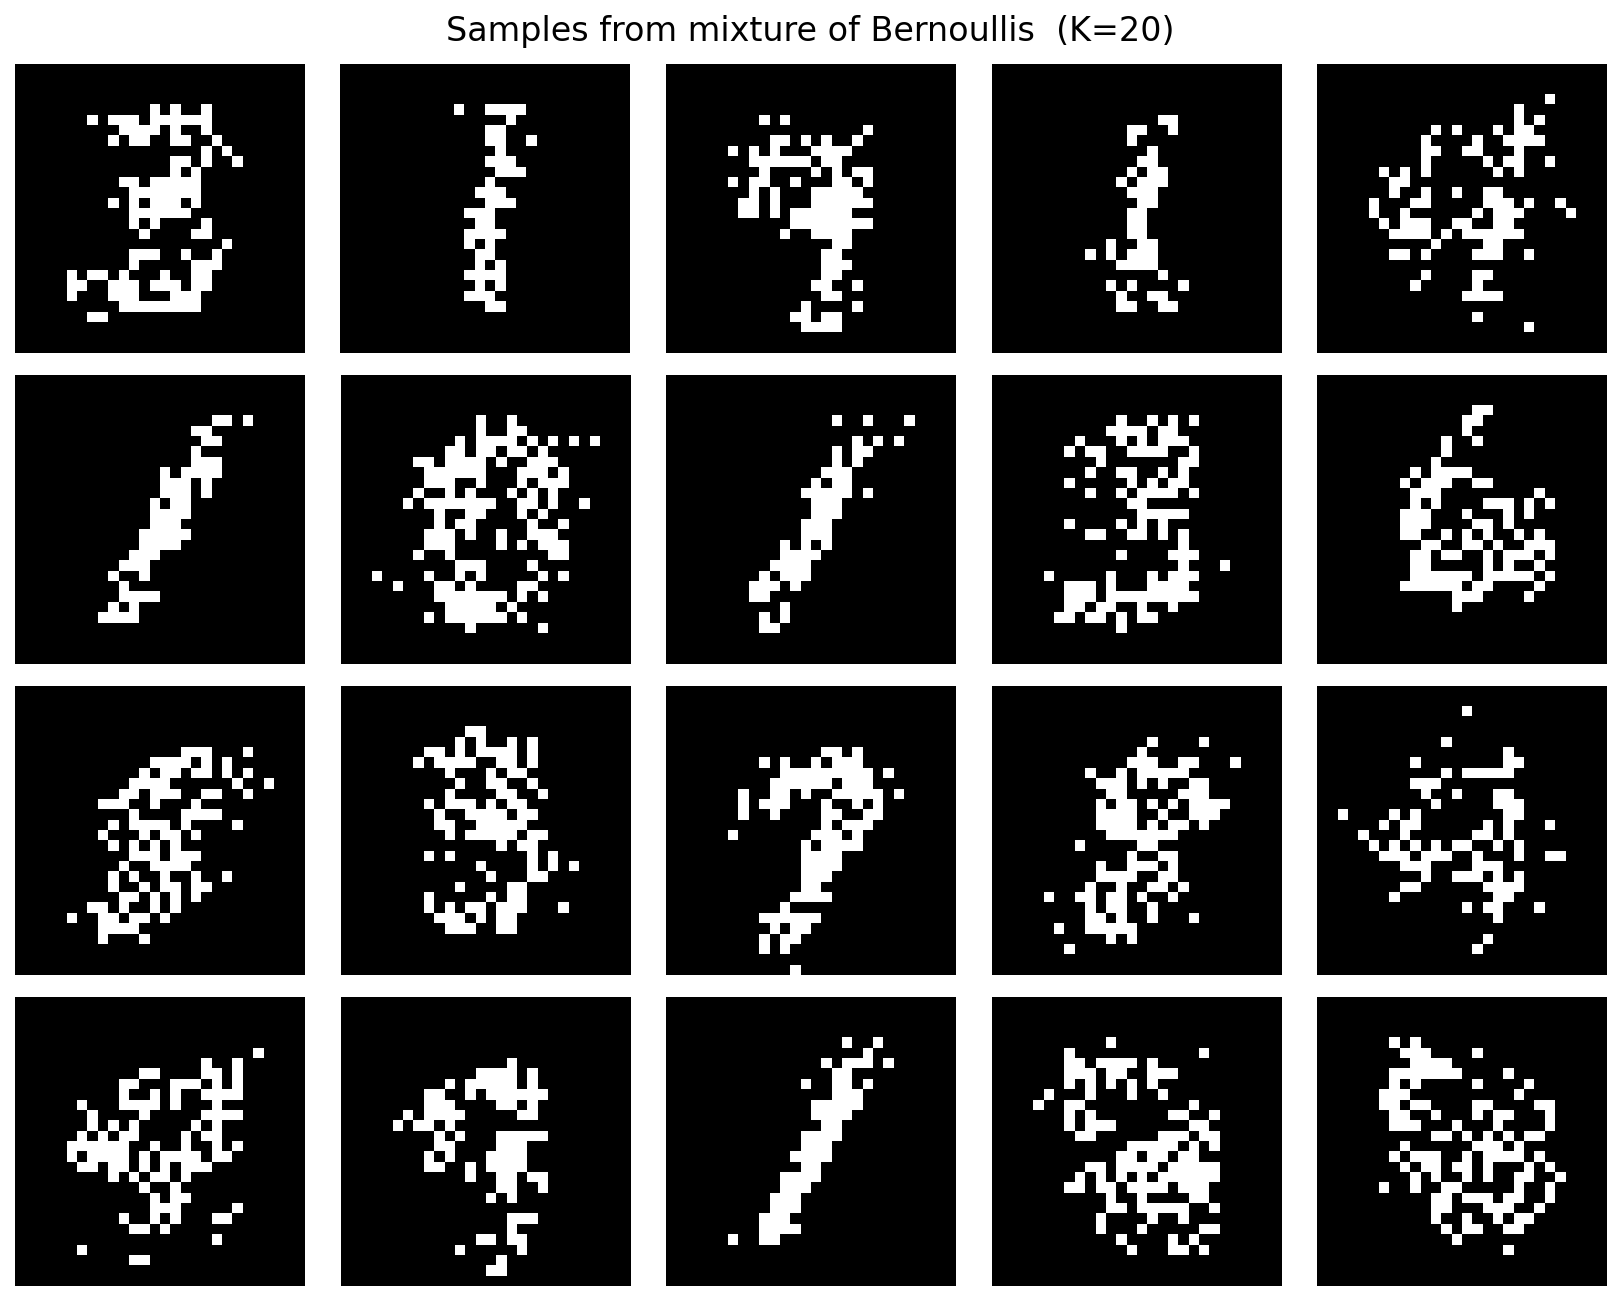
\includegraphics[width=0.62\textwidth]{samples_K20.png}
  \caption{Samples from the \(K=20\) mixture. Even when a mean
    \(p^{(k)}\) looks like a clean digit, a sample looks like a speckled
    ghost of that digit.}
\end{figure}

With \(K=5\) the means already mix several classes, so samples are
noisy blobs. With \(K=10\) and \(K=20\) the means look more digit-like,
but samples remain speckled. Extra clusters reduce between-digit mixing;
they do not restore spatial structure. The fitted \(p^{(k)}\) are useful
as cluster centroids. As a generative model of MNIST the mixture of
independent Bernoullis is misspecified: it can match per-pixel
marginals within a cluster, but not the joint distribution of pixels.

%%%%%%%%%%%%%%%%%%%%%%%%%%%%%%%%%%%%%%%%%%%%%%%%%%%%%%%%%%%%%%%%%%%%%%%%
\section{Problem 4: NICE vs.\ VAE on MNIST (10 points)}
%%%%%%%%%%%%%%%%%%%%%%%%%%%%%%%%%%%%%%%%%%%%%%%%%%%%%%%%%%%%%%%%%%%%%%%%

\begin{question}
We will now compare the performance of a NICE and VAE implementation on MNIST, again using the repository \url{https://github.com/EugenHotaj/pytorch-generative}, which you will need to clone into your working directory.
\begin{enumerate}
  \item[(a)] Train the NICE model for \(50\) epochs and batch size \(256\) (keep the other parameters at default). Visualize a few samples from the model and comment on the result.
  \item[(b)] Repeat the process with the VAE model with the same parameters as above (remember that the setups for the models and loss functions are different). Does this model generate more plausible samples? Explain.
  \item[(c)] Considering these two models as well as the EM-based generation described in Problem~3(e), which one would be more suitable for this type of data? Your answer may consider runtime, generative expressiveness/power, simplicity, or any other factors you consider relevant.
\end{enumerate}
\end{question}

Both models were trained from
\texttt{pytorch-generative}\footnote{\url{https://github.com/EugenHotaj/pytorch-generative}}
for \(50\) epochs with batch size \(256\), leaving architecture,
optimizer, and loss at the repository defaults. NICE is trained on
\emph{dequantized} \(28\times 28\) MNIST (continuous density). The VAE
is trained on \emph{dynamically binarized} \(32\times 32\) MNIST
(Bernoulli decoder). Those data and loss setups differ by design.

\begin{center}
\begin{tabular}{@{}lrrr@{}}
  \toprule
  Model & Params & Train time (CPU) & Final eval \\
  \midrule
  NICE & \(19.2\)M & \(30.7\) min & NLL \(=-1972\) nats/image (started at \(+943\)) \\
  VAE  & \(0.97\)M & \(78.6\) min & \(-\)ELBO (loss) \(=93.7\) nats/image (recon \(72.0\), KL \(21.7\)) \\
  \bottomrule
\end{tabular}
\end{center}

Both numbers are per image, in nats. The NICE NLL is negative because it
is a \emph{continuous} density on dequantized pixels scaled to
\([0,1)^{784}\): each unit cube of pixel values is squeezed into a cell of
volume \(256^{-784}\), so densities far above 1 are expected. Adding
\(784\log256\approx4347\) nats converts it to an upper bound of about
\(2375\) nats (\(4.37\) bits/dim) on the discrete NLL. The VAE number is
the negative ELBO on binarized \(32\times32\) images, a different random
variable, so the two are not directly comparable.

\subsection{NICE}

NICE is a normalizing flow: additive coupling layers plus a diagonal
scaling, trained by exact logistic-prior log-likelihood. Sampling is one
inverse pass \(z\sim p(z)\mapsto x=f^{-1}(z)\).

\begin{figure}[H]
  \centering
  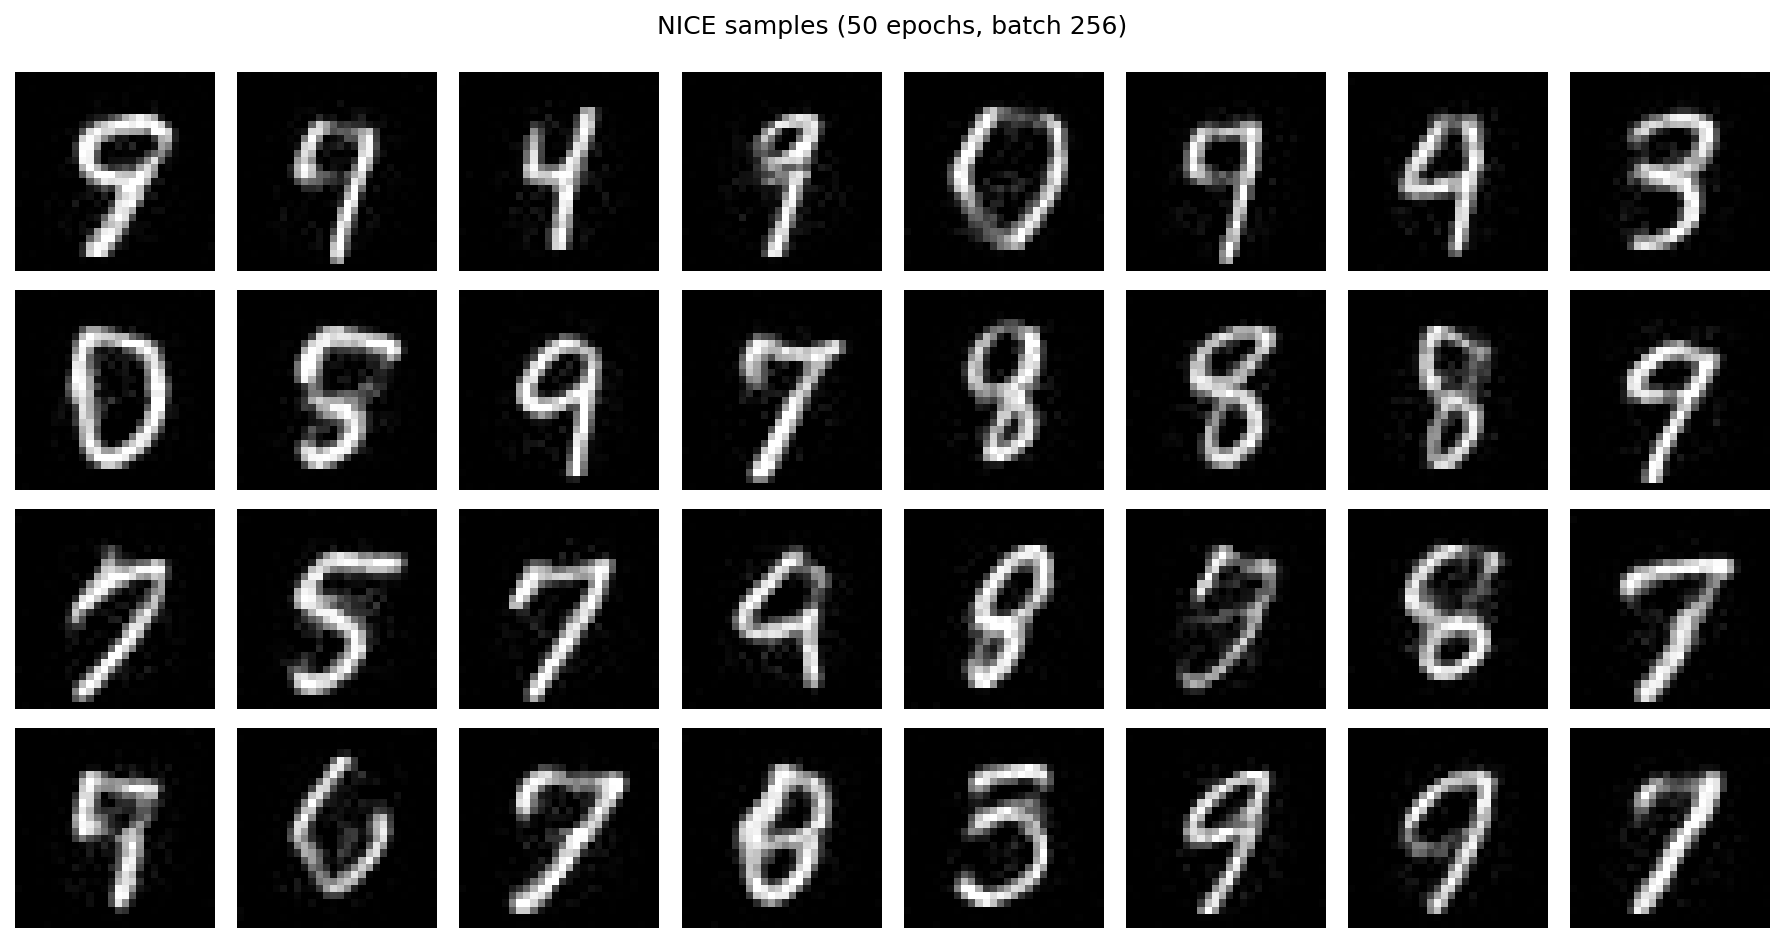
\includegraphics[width=0.85\textwidth]{nice_samples.png}
  \caption{NICE samples after \(50\) epochs. Recognizable digits with
    coherent strokes; a bit soft (continuous dequantized pixels), with a
    few malformed shapes (e.g.\ \(4/9\) confusion).}
\end{figure}

Each coupling block is invertible and mixes half of the pixels as a
function of the other half, so spatial dependence is in the model.
Fifty epochs were enough for the loss to drop steadily and flatten near
\(-1970\).

\subsection{VAE}

The repository VAE maximizes the ELBO with a convolutional
encoder/decoder and a factorized Bernoulli reconstruction term. The
official sampler draws \(x\sim\mathrm{Bernoulli}(\sigma(\mathrm{decoder}(z)))\).

\begin{figure}[H]
  \centering
  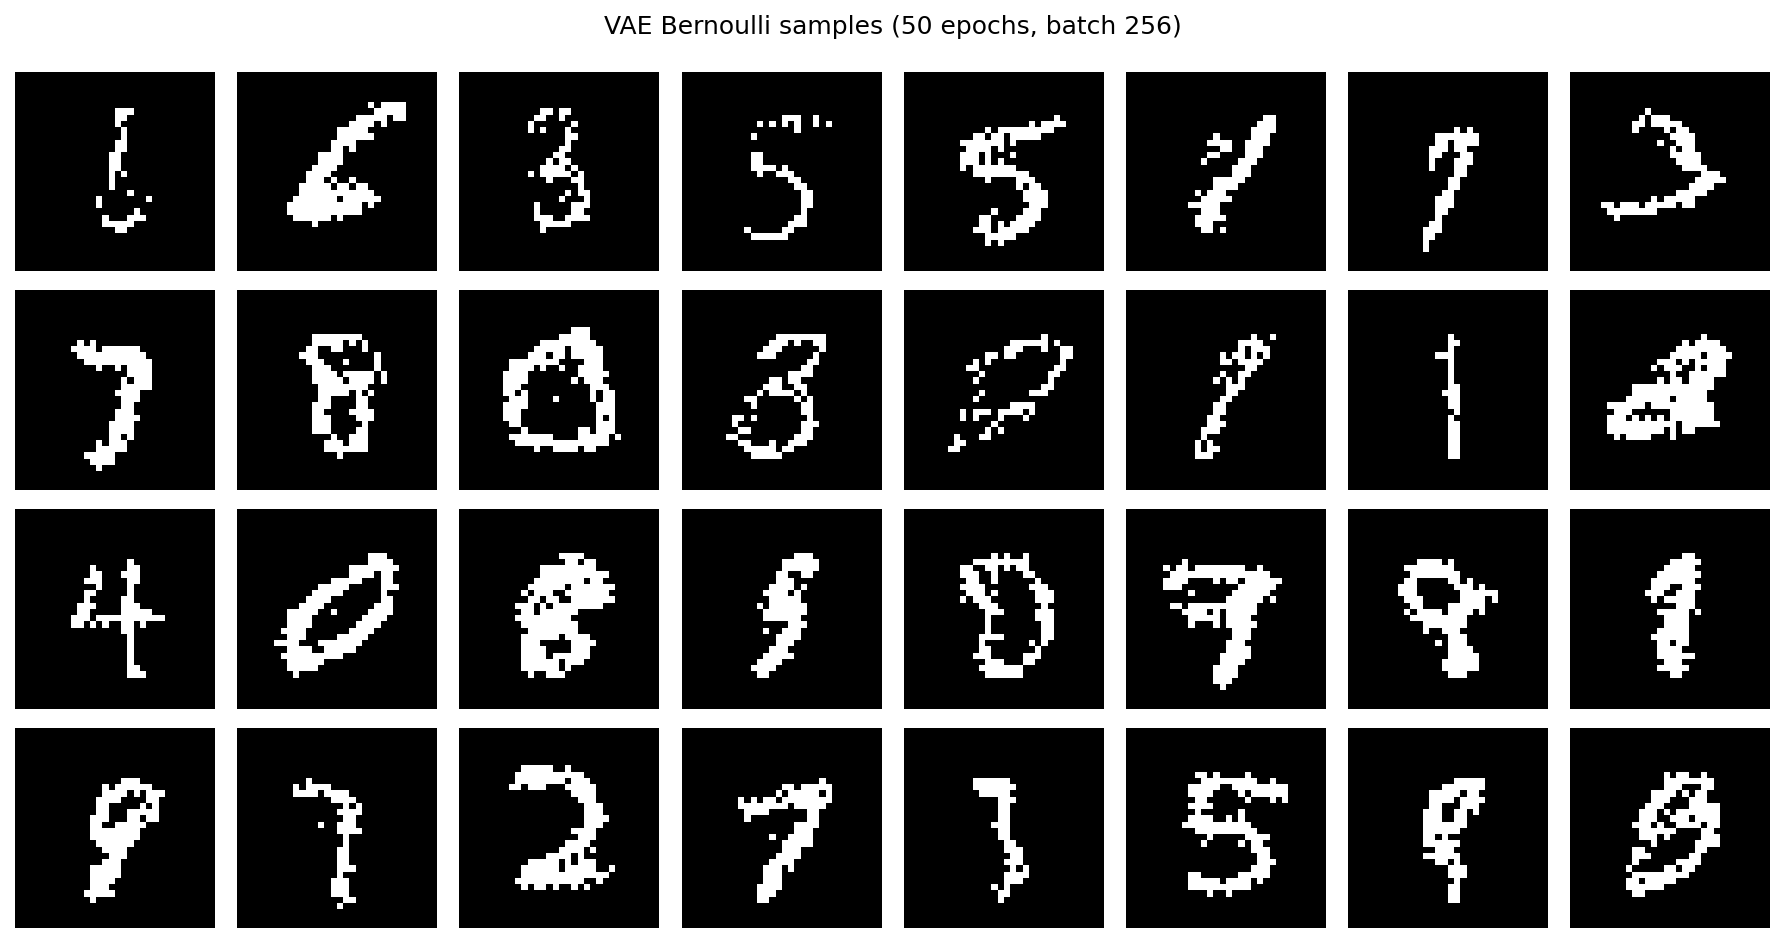
\includegraphics[width=0.85\textwidth]{vae_samples.png}
  \caption{VAE Bernoulli samples. Digit identities are often clear, but
    edges are blotchy: the same pixel-independence artifact as in the EM
    generator, now with a neural mean \(\hat p(z)\).}
\end{figure}

\begin{figure}[H]
  \centering
  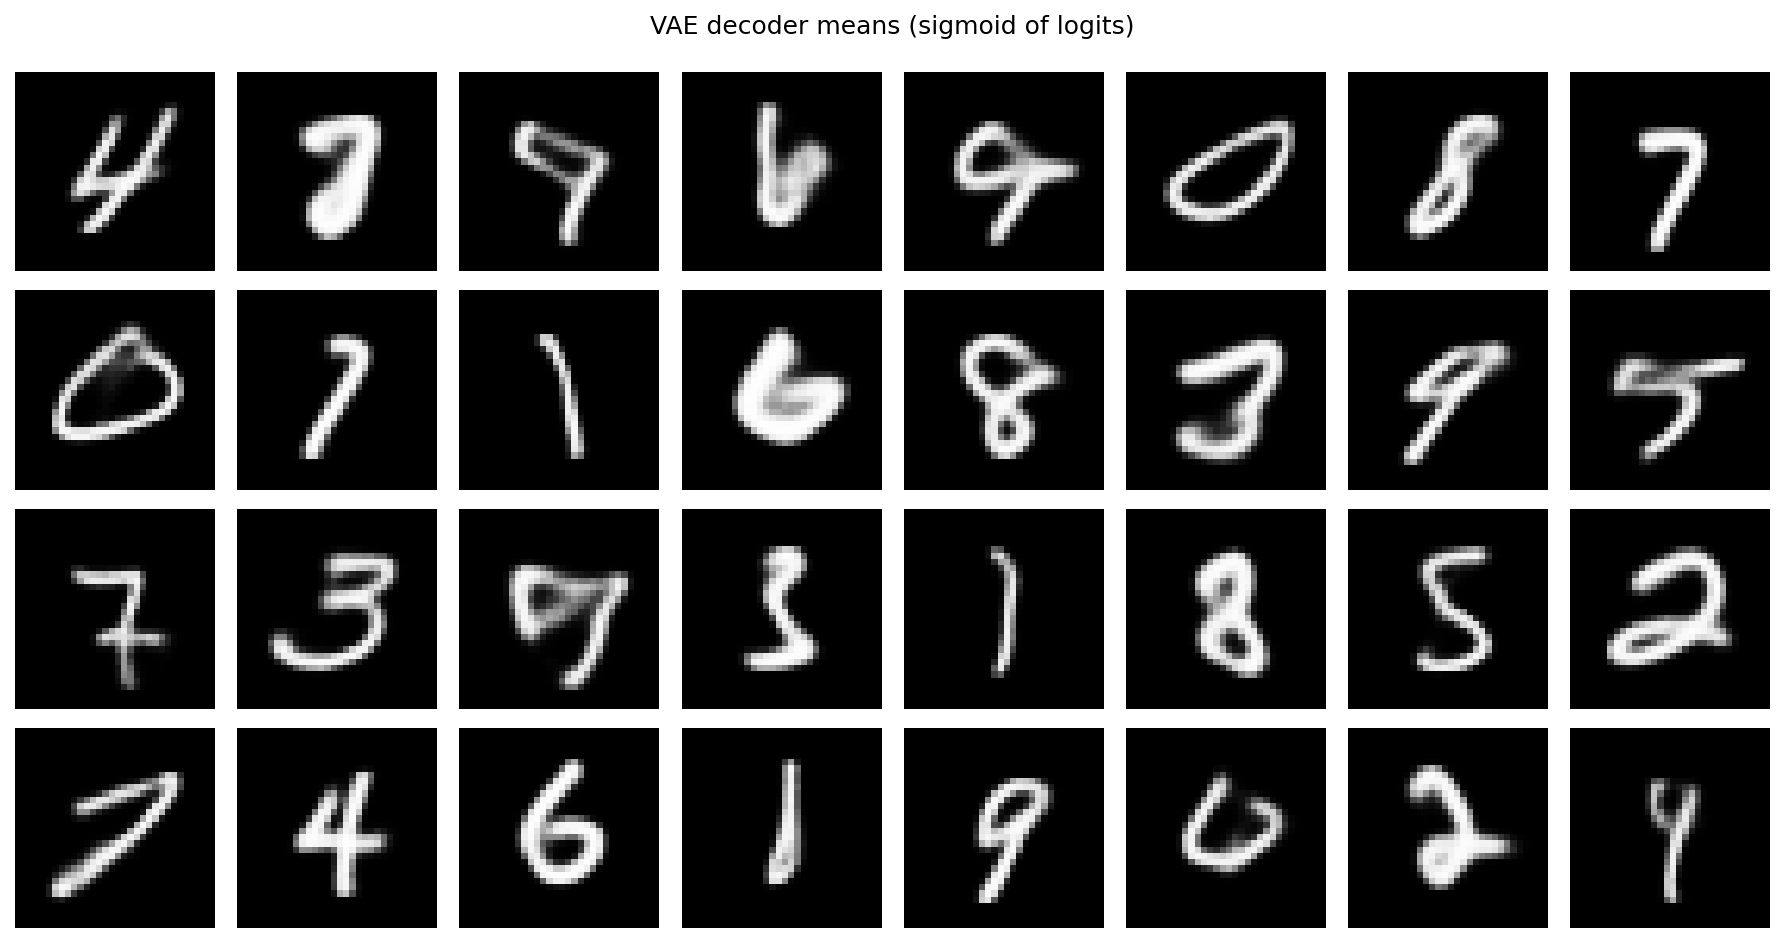
\includegraphics[width=0.85\textwidth]{vae_samples_means.png}
  \caption{VAE decoder means \(\sigma(\mathrm{decoder}(z))\). Smoother and
    more digit-like than the Bernoulli samples, but still blurrier than
    NICE.}
\end{figure}

VAE samples are more plausible than the mixture of Bernoullis, but
\emph{not} more plausible than NICE. NICE wins on stroke structure
because it models a joint density over all pixels. The VAE decoder is
\[
  p(x\mid z)=\prod_d \mathrm{Bernoulli}\bigl(x_d;\hat p_d(z)\bigr),
\]
so even a good latent code yields speckle when sampled.

Two training notes: epochs \(1\)--\(3\) had posterior collapse
(\(\mathrm{KL}\approx 0\)); the KL jumped at epoch \(4\) and stayed
around \(20\)--\(22\). The official recipe trains this VAE for \(457\)
epochs, so \(50\) is undertrained relative to that default, which shows
up as remaining blur.

\subsection{Which model is more suitable?}

Among EM, VAE, and NICE, NICE is the best \emph{generator} for this
data. MNIST is high-dimensional and spatially dependent. A model that
represents \(p(x)\) as a joint over pixels looks like handwriting; a
model that treats pixels as independent given a discrete or continuous
code looks like static.

\begin{center}
\small
\begin{tabular}{@{}>{\raggedright\arraybackslash}p{2.9cm}
                >{\raggedright\arraybackslash}p{3.9cm}
                >{\raggedright\arraybackslash}p{3.7cm}
                >{\raggedright\arraybackslash}p{3.7cm}@{}}
  \toprule
  & Mixture of Bernoullis (EM) & VAE & NICE \\
  \midrule
  Model
    & \(\sum_k\pi_k\prod_d\mathrm{Bern}(p_d^{(k)})\)
    & \(\int p(x\mid z)p(z)\,dz\), factorized \(p(x\mid z)\)
    & invertible \(x=f^{-1}(z)\) \\
  Pixel dependence
    & none given \(k\) & none given \(z\) & yes (coupling nets) \\
  Samples
    & unusable speckle
    & noisy but class-recognizable
    & coherent digits \\
  Likelihood & exact (simple) & ELBO only & exact \\
  Train time (CPU)
    & seconds
    & \(78.6\) min (50 epochs)
    & \(30.7\) min (50 epochs) \\
  Other uses
    & clustering, mean digits
    & latent interpolation, compression
    & density estimation, exact NLL \\
  \bottomrule
\end{tabular}
\end{center}

EM is appropriate for clustering, not generation. VAE is preferable if
the goal is a low-dimensional latent for interpolation or reconstruction:
sampling is cheap and the network is small (\(\sim 1\)M vs.\ \(19\)M).
It is the wrong default if sample fidelity is the metric, because
reverse KL and a factorized decoder both fight sharp, multimodal images.
For generating MNIST-like images among these three, use NICE.

%%%%%%%%%%%%%%%%%%%%%%%%%%%%%%%%%%%%%%%%%%%%%%%%%%%%%%%%%%%%%%%%%%%%%%%%
\section{Problem 5: Simple Flow Models (10 points)}
%%%%%%%%%%%%%%%%%%%%%%%%%%%%%%%%%%%%%%%%%%%%%%%%%%%%%%%%%%%%%%%%%%%%%%%%

\begin{question}
\begin{enumerate}
  \item[(a)] Let \(X\) be a Cauchy random variable with pdf \(1/(\pi(1+x^2))\). Find the distribution of \(1/X\).
  \item[(b)] Let \(Y\) be a normal random variable with parameters \(\mu\) and \(\sigma\). Find the density of \(e^Y\).
  \item[(c)] We choose a point \(P\) uniformly on \([0,2]^2\). Denote the distance of \(P\) from the point \((1,1)\) by \(Z\). Find the density of \(Z\).
\end{enumerate}
\end{question}

If \(Z=f(X)\) is invertible and smooth, then
\begin{equation}
  p_Z(z)
  =p_X\bigl(f^{-1}(z)\bigr)
  \Bigl|\det\frac{\partial f^{-1}}{\partial z}\Bigr|.
\end{equation}

\subsection{\texorpdfstring{\(Z=1/X\) for standard Cauchy \(X\)}{Z = 1/X for standard Cauchy X}}

Let \(X\) have density \(1/(\pi(1+x^2))\). The map \(f(x)=1/x\) is a
\(C^\infty\) bijection \(\R\setminus\{0\}\to\R\setminus\{0\}\) (and
\(P(X=0)=0\)). Inverse \(x=1/z\), Jacobian \(|dx/dz|=1/z^2\). Hence
\begin{equation}
  p_Z(z)
  =\frac{1}{\pi\bigl(1+(1/z)^2\bigr)}\cdot\frac{1}{z^2}
  =\frac{1}{\pi(1+z^2)}.
\end{equation}
Thus \(1/X\) is again standard Cauchy: inversion is a normalizing flow
that leaves this density invariant.

\subsection{\texorpdfstring{\(Z=e^Y\) for \(Y\sim\mathcal{N}(\mu,\sigma^2)\)}{Z = e^Y for Y normal}}

The map \(f(y)=e^y\) sends \(\R\) onto \((0,\infty)\), with inverse
\(y=\log z\) and \(|dy/dz|=1/z\). For \(z>0\),
\begin{equation}
  p_Z(z)
  =\frac{1}{z\,\sigma\sqrt{2\pi}}
  \exp\Biggl(-\frac{(\log z-\mu)^2}{2\sigma^2}\Biggr),
\end{equation}
and \(p_Z(z)=0\) for \(z\le 0\). This is the log-normal density
\(\mathrm{LogNormal}(\mu,\sigma^2)\). Exponentiation is the flow that
sends a Gaussian latent to a positive observation.

\subsection{Distance from a uniform point in the square to its center}

Let \(P\sim\mathrm{Unif}([0,2]^2)\) and \(Z=\|P-(1,1)\|_2\). Shift to
\(U=X-1\), \(V=Y-1\), so \((U,V)\) is uniform on the square
\([-1,1]^2\) of area \(4\), and
\[
  Z=\sqrt{U^2+V^2}\in[0,\sqrt{2}].
\]
The density is the arc length \(L(z)\) of \(\{u^2+v^2=z^2\}\) inside the
square, divided by \(4\):
\[
  p_Z(z)=L(z)/4.
\]

\begin{itemize}
  \item For \(0\le z\le 1\) the circle lies entirely in the square, so
    \(L(z)=2\pi z\) and \(p_Z(z)=\pi z/2\).
  \item For \(1<z\le\sqrt{2}\) the circle is cut by the four sides. In
    each quadrant the surviving arc runs between angles \(\theta\) and
    \(\pi/2-\theta\), where \(\theta=\arccos(1/z)\). Four copies give
    total angle \(2\pi-8\arccos(1/z)\), hence
    \[
      p_Z(z)
      =z\Bigl(\tfrac{\pi}{2}-2\arccos\tfrac{1}{z}\Bigr).
    \]
    Equivalently \(\arccos(1/z)=\arctan\sqrt{z^2-1}\). At the endpoints
    this matches: \(p_Z(1)=\pi/2\) and \(p_Z(\sqrt{2})=0\).
\end{itemize}
Piecewise,
\begin{equation}
  p_Z(z)=
  \begin{cases}
    \dfrac{\pi z}{2},
      & 0\le z\le 1,\\[10pt]
    z\Bigl(\dfrac{\pi}{2}-2\arccos\dfrac{1}{z}\Bigr),
      & 1<z\le\sqrt{2},\\[10pt]
    0,
      & \text{otherwise.}
  \end{cases}
\end{equation}
This transformation is not a global diffeomorphism of \(\R^2\) (many
points share the same radius), so the one-dimensional Jacobian formula
of (a)--(b) does not apply directly; the density comes from the coarea
formula / the area of \(\{Z\le z\}\) inside the square.

%%%%%%%%%%%%%%%%%%%%%%%%%%%%%%%%%%%%%%%%%%%%%%%%%%%%%%%%%%%%%%%%%%%%%%%%
\section{Problem 6: Jacobian of the Leaky Flow (10 points)}
%%%%%%%%%%%%%%%%%%%%%%%%%%%%%%%%%%%%%%%%%%%%%%%%%%%%%%%%%%%%%%%%%%%%%%%%

\begin{question}
The leaky ReLU is defined as \(\mathrm{LReLU}[z]=0.1z\) for \(z<0\) and \(\mathrm{LReLU}[z]=z\) for \(z>0\). Write an expression for the inverse of the leaky ReLU. Write an expression for the inverse absolute determinant of the Jacobian \(\bigl|\partial\mathbf{f}[\mathbf{z}]/\partial\mathbf{z}\bigr|^{-1}\) for an elementwise transformation \(\mathbf{x}=\mathbf{f}[\mathbf{z}]\) of the multivariate variable \(\mathbf{z}\), where
\[
  \mathbf{f}[\mathbf{z}]
  =\bigl[\mathrm{LReLU}[z_1],\mathrm{LReLU}[z_2],\ldots,\mathrm{LReLU}[z_n]\bigr]^\top.
\]
\end{question}

The leaky ReLU
\[
  \mathrm{LReLU}[z]
  =
  \begin{cases}
    0.1z & z<0,\\
    z    & z>0
  \end{cases}
\]
is piecewise linear and strictly increasing, hence invertible almost
everywhere (the kink at \(0\) has measure zero).

\subsection{Inverse}

\[
  \mathrm{LReLU}^{-1}[x]
  =
  \begin{cases}
    10x & x<0,\\
    x   & x\ge 0.
  \end{cases}
\]
If \(z<0\) then \(x=0.1z\) so \(z=10x\); if \(z>0\) then \(x=z\).
Coordinatewise,
\[
  \mathbf{z}
  =\mathbf{f}^{-1}[\mathbf{x}]
  =\bigl[\mathrm{LReLU}^{-1}[x_1],\ldots,\mathrm{LReLU}^{-1}[x_n]\bigr]^\top.
\]

\subsection{Inverse absolute Jacobian determinant}

Because \(\mathbf{f}\) acts independently on each coordinate,
\(\partial\mathbf{f}/\partial\mathbf{z}\) is diagonal:
\[
  \frac{\partial f_i}{\partial z_j}
  =\delta_{ij}\,
  \begin{cases}
    0.1 & z_i<0,\\
    1   & z_i>0.
  \end{cases}
\]
The determinant is the product of the diagonal entries, all positive:
\begin{equation}
  \Bigl|\frac{\partial\mathbf{f}[\mathbf{z}]}{\partial\mathbf{z}}\Bigr|
  =\prod_{i=1}^n
  \begin{cases}
    0.1 & z_i<0,\\
    1   & z_i>0
  \end{cases}
  =0.1^{\,n_-(\mathbf{z})},
\end{equation}
where \(n_-(\mathbf{z})=\sum_{i=1}^n\ind_{z_i<0}\) is the number of
negative coordinates. Therefore
\begin{equation}
  \Bigl|\frac{\partial\mathbf{f}[\mathbf{z}]}{\partial\mathbf{z}}\Bigr|^{-1}
  =10^{\,n_-(\mathbf{z})}
  =\prod_{i=1}^n
  \bigl(10\cdot\ind_{z_i<0}+\ind_{z_i>0}\bigr).
\end{equation}
Signs are preserved by \(\mathbf{f}\), so the same quantity in
\(x\)-space is \(10^{n_-(\mathbf{x})}\). In a flow this is the volume
correction
\begin{equation}
  p(\mathbf{x})
  =p(\mathbf{z})\,
  \Bigl|\frac{\partial\mathbf{f}[\mathbf{z}]}{\partial\mathbf{z}}\Bigr|^{-1}
  =p\bigl(\mathbf{f}^{-1}[\mathbf{x}]\bigr)\,
  10^{\,n_-(\mathbf{x})}.
\end{equation}

%%%%%%%%%%%%%%%%%%%%%%%%%%%%%%%%%%%%%%%%%%%%%%%%%%%%%%%%%%%%%%%%%%%%%%%%
\section{GDL-Bench Challenge Problem (20 points)}
%%%%%%%%%%%%%%%%%%%%%%%%%%%%%%%%%%%%%%%%%%%%%%%%%%%%%%%%%%%%%%%%%%%%%%%%

\begin{question}
As part of each homework, you will contribute one candidate problem to GDL-Bench, a benchmark for evaluating the reasoning capabilities of current AI systems in generative and geometric deep learning. For this homework, design one original challenge problem related to one or more of the topics covered in this assignment. The problem should require genuine mathematical, conceptual, algorithmic, or implementation-level reasoning, and should not be answerable by simply recalling a definition or looking up a fact.
\begin{enumerate}
  \item[(a)] \textbf{Challenge problem.} Write the exact problem as you would like it to appear in GDL-Bench. It must be original, self-contained, technically well-defined, and unambiguous.
  \item[(b)] \textbf{Gold answer and solution.} Provide the correct final answer together with a concise but complete solution, enough for another student or instructor to independently verify the answer. Whenever possible, design the problem so that the final answer can be objectively checked.
  \item[(c)] \textbf{What does the problem test?} Topic; problem type (derivation, conceptual reasoning, counterexample, numerical, coding/debugging, algorithm design, or other); and the core insight in 1--3 sentences, including why a solver with only superficial knowledge might struggle.
  \item[(d)] \textbf{Test AI systems.} Only after the problem and solution are finalized, give the exact same problem to at least two current AI models, with no extra hints and without the solution. For each model report the name/version, whether the answer was Correct, Partially Correct, or Incorrect, and a 1--3 sentence explanation of any important error. A problem does not need to defeat the models to receive full credit.
\end{enumerate}
Quality bar: original, relevant, self-contained, unambiguous, verifiable, and reasoning-intensive. Grading: relevance and originality (4); technical correctness (6); clarity (4); depth of reasoning (4); complete metadata and AI evaluation (2).
\end{question}

The full, agent-runnable version of this problem (data, task statement,
reference solution, and automated tests) is in
\texttt{gdlbench\_submission/}. The statement below is the text of
\texttt{task/TASK.md}.

\subsection{(a) Challenge problem}

\textbf{Which of three MNIST generative models is actually best?}

The file \texttt{data/images.csv} holds 1000 MNIST digits, one image per row,
784 columns (row-major \(28\times28\)). Each entry is the raw 8-bit pixel value
\(k\in\{0,1,\dots,255\}\).

Three generative models were evaluated on \emph{exactly these 1000 images}.
Each team reported a single number, computed with the preprocessing code
below. In all snippets, \texttt{to\_tensor} maps a uint8 image to float32 by
dividing by 255 (pixel \(k\) becomes \(k/255\)), \texttt{torch.rand\_like}
draws i.i.d.\ \(\mathrm{Uniform}[0,1)\) noise, and a fresh noise or Bernoulli
draw is made every time an image is used. Reported numbers are exact averages
over the 1000 images and over all of this randomness. All logarithms are
natural.

\medskip\noindent\textbf{Model A: normalizing flow.}
\begin{verbatim}
x = to_tensor(img)                       # shape (784,)
y = (x * 255 + torch.rand_like(x)) / 256
score = flow_A.log_prob(y)               # log-density of y under flow A
\end{verbatim}
Reported: mean \texttt{score} \(=1972.0\) nats per image.

\medskip\noindent\textbf{Model B: normalizing flow in logit space (\(\lambda=0.05\)).}
\begin{verbatim}
x = to_tensor(img)                       # shape (784,)
y = x + torch.rand_like(x) / 256
s = lam + (1 - 2 * lam) * y
y_prime = torch.log(s) - torch.log1p(-s)
score = flow_B.log_prob(y_prime)         # log-density of y_prime under flow B
\end{verbatim}
Reported: mean \texttt{score} \(=-150.0\) nats per image, with \texttt{lam = 0.05}.

\medskip\noindent\textbf{Model C: VAE with a Bernoulli decoder.}
\begin{verbatim}
x = to_tensor(img).view(1, 28, 28)
b = torch.bernoulli(x)                   # dynamic binarization
b = F.pad(b, (2, 2, 2, 2))               # zero-pad to 1 x 32 x 32
logits, kl = vae(b)
loss = F.binary_cross_entropy_with_logits(logits, b, reduction="sum") + kl
\end{verbatim}
Reported: mean \texttt{loss} \(=93.7\) nats per image.

Both flows have densities that are strictly positive and finite on all of
their input space. Treat every reported number as exact.

\medskip\noindent\textbf{The comparison.} For a model that assigns probability
\(P(x)\) to each 8-bit image \(x\), the quantity of interest is
\[
  \mathrm{bpd}=-\frac{1}{784}\cdot\frac{1}{1000}\sum_{x}\log_2 P(x)
\]
over the 1000 images. For a continuous model, \(P(x)\) is the probability its
density assigns to the set of inputs that image \(x\) can be turned into by the
model's own preprocessing and noise. The reported numbers do not give bpd
directly, so for each model use the standard dequantization (Jensen) upper
bound on bpd implied by the reported number, whenever the reported number
implies one.

\medskip\noindent\textbf{Report:}
\begin{enumerate}
  \item \texttt{bpd\_A}: the upper bound on bpd for Model A.
  \item \texttt{bpd\_B}: the upper bound on bpd for Model B (\(\lambda=0.05\)),
        or \texttt{null} if Model B's reported number does not imply a valid
        upper bound on its bpd.
  \item \texttt{better}: \texttt{"A"} or \texttt{"B"}, whichever flow has the
        lower bound.
  \item \texttt{lambda\_min}: Model B's pipeline is only well defined (finite
        \texttt{y\_prime} for every possible 8-bit image and every noise draw)
        for some values of \(\lambda\in(0,1/2)\). Report the smallest such
        \(\lambda\).
  \item \texttt{lambda\_star}: suppose Model B's team had not stated
        \(\lambda\). Keeping the reported mean score fixed at \(-150.0\) and
        the pipeline otherwise unchanged, report the
        \(\lambda\in[\texttt{lambda\_min},1/2)\) at which Model B's bound
        exactly equals Model A's.
  \item \texttt{bpd\_C\_own}: Model C's reported number expressed in bits per
        dimension of the random variable that Model C actually models.
  \item \texttt{bpd\_C\_8bit}: an upper bound on bpd for Model C computed from
        its reported number, or \texttt{null} if it implies no such bound.
\end{enumerate}
Answers go in \texttt{task/results/answer.json}, floats to at least 6
significant figures. Tolerances: bpd values \(\pm10^{-3}\) bits/dim,
\texttt{lambda\_min} \(10^{-6}\) relative, \texttt{lambda\_star}
\(\pm5\times10^{-5}\), \texttt{bpd\_C\_own} \(\pm10^{-4}\); \texttt{better}
and any \texttt{null} must match exactly.

The reported numbers for A and C are the ones from our own runs in
Problem~4 (NICE and VAE in \texttt{pytorch-generative}, whose pipelines are
exactly those shown). Model B is a hypothetical variant with a common
\texttt{/255} preprocessing slip.

\subsection{(b) Gold answer and solution}

\begin{center}
\begin{tabular}{@{}ll@{}}
\toprule
Key & Gold answer\\
\midrule
\texttt{bpd\_A} & \(4.371180\)\\
\texttt{bpd\_B} & \(4.283594\)\\
\texttt{better} & B\\
\texttt{lambda\_min} & \(1/258\approx0.00387597\)\\
\texttt{lambda\_star} & \(0.053360\)\\
\texttt{bpd\_C\_own} & \(0.132012\)\\
\texttt{bpd\_C\_8bit} & \texttt{null}\\
\bottomrule
\end{tabular}
\end{center}

\paragraph{Common bound.} Let \(D=784\). If a model's preprocessing sends
image \(x\) to a set \(B_x\) of volume \(V_x\) in the space \(y\) where its
(pre-logit) density \(p_Y\) lives, then
\(P(x)=\int_{B_x}p_Y=V_x\,\E_u[p_Y(y)]\), and by Jensen
\[
  -\log P(x)\le-\E_u[\log p_Y(y)]-\log V_x .
\]
For A and B each bin is a cube of side \(1/256\), so \(V_x=256^{-D}\) and
\[
  \mathrm{bpd}\le 8-\frac{\E[\log p_Y]}{D\ln 2}.
\]

\paragraph{Model A.} \(y=(k+u)/256\), bins tile \([0,1)^D\), and
\(\E[\log p_Y]=\ell_A\):
\(\mathrm{bpd}_A=8-1972/(784\ln2)=4.371180\).

\paragraph{Model B: validity.} Here \(y=k/255+u/256\). The bins have width
\(1/256\) but sit on a \(1/255\) grid, so they are disjoint with small gaps
and \(\sum_xP(x)<1\) (true for A as well, since both flows put mass outside
the bins). A deficient model still gives a valid Jensen bound, and each bin
still has volume \(256^{-D}\), so the bound is valid and uses \(D\log256\),
not \(D\log255\).

\paragraph{Model B: value.} By change of variables through the elementwise logit,
\[
  \log p_Y(y)=\log p_B(y')+\sum_{d}\Bigl[\log(1-2\lambda)-\log s_d-\log(1-s_d)\Bigr],
  \qquad s=\lambda+(1-2\lambda)\Bigl(\tfrac{k}{255}+\tfrac{u}{256}\Bigr).
\]
The Jacobian term depends on each pixel's value and on \(u\), so it must be
averaged over the data and the noise. For pixel value \(k\), \(s\) is uniform
on \([a,a+c]\) with \(a=\lambda+(1-2\lambda)k/255\), \(c=(1-2\lambda)/256\),
so with \(F(t)=t\log t-t\),
\[
  \E_u[\log s]=\frac{F(a+c)-F(a)}{c},\qquad
  \E_u[\log(1-s)]=\frac{F(1-a)-F(1-a-c)}{c}.
\]
Summing this 256-entry table against the pixel-value histogram of
\texttt{images.csv} gives a mean log-Jacobian \(J(0.05)=2169.597\) nats per
image. Hence
\(\mathrm{bpd}_B=8-(-150+2169.597)/(784\ln2)=4.283594<\mathrm{bpd}_A\):
B is better, even though its raw score is about 2100 nats lower.

\paragraph{\(\lambda_{\min}\).} Pixel 255 with \(u\to1\) gives
\(y\to1+1/256\). A finite logit needs
\(\lambda+(1-2\lambda)(1+1/256)\le1\) (strict \(s<1\) then holds because
\(u<1\)), i.e.\ \(\lambda\ge1/258\). The lower end \(s\ge\lambda>0\) never
binds.

\paragraph{\(\lambda^\star\).} Equating the two bounds cancels
\(D\log256\) and leaves \(J(\lambda)=\ell_A-\ell_B=2122\). Both
\(\log(1-2\lambda)\) and \(-\log s(1-s)\) decrease in \(\lambda\), so
\(J\) is decreasing on \([1/258,1/2)\) and the root is unique; bisection gives
\(\lambda^\star=0.053360\). B wins only because its \(\lambda=0.05\) sits just
below the break-even point.

\paragraph{Model C.} The loss is \(-\mathrm{ELBO}\ge-\log p_C(b)\) for the
binary \(32\times32\) variable \(b\) (1024 dimensions, 240 of them zero
padding), so \(\mathrm{bpd}_{C,\text{own}}=93.7/(1024\ln2)=0.132012\). It says
nothing about \(P(x)\) for the 8-bit image: binarization is a random,
many-to-one map (many 8-bit images can give the same \(b\), and each image
gives many \(b\)), not a dequantization, so no bound on the 8-bit NLL follows
and \texttt{bpd\_C\_8bit} is \texttt{null}. Comparing \(0.13\) with \(4.3\)
bits/dim is meaningless.

\paragraph{Verification.} The reference script
(\texttt{gt\_code/reference\_solution.py}) computes
the closed form. An independent Monte Carlo solve (10 noise draws per pixel,
bisection for \(\lambda^\star\)) matches every value and passes all 8 tests.
Each of the following mistakes fails at least one test:
\begin{center}
\begin{tabular}{@{}ll@{}}
\toprule
Mistake & Effect\\
\midrule
Use the \texttt{/256} pipeline for B (miss the slip) & \(\mathrm{bpd}_B=4.290814\), \(\lambda^\star=0.053092\)\\
Use \(D\log255\) because of the \texttt{/255} & \(\mathrm{bpd}_B=4.277947\)\\
Declare B's bound invalid because bins do not tile & \texttt{bpd\_B = null}\\
Divide C's loss by 784 (ignore padding) & \(\mathrm{bpd}_{C,\text{own}}=0.172415\)\\
Report C's number as an 8-bit bpd & \texttt{bpd\_C\_8bit} \(\ne\) \texttt{null}\\
Compare raw scores, or use a constant logit Jacobian & wrong \texttt{better}\\
\bottomrule
\end{tabular}
\end{center}

\subsection{(c) What does the problem test?}

\begin{itemize}
  \item \textbf{Topic:} normalizing flows (change of variables,
        dequantization), VAEs and the ELBO, likelihood evaluation of
        generative models on discrete data.
  \item \textbf{Problem type:} coding/debugging (reading preprocessing code),
        derivation, and numerical computation.
  \item \textbf{Core insight:} a reported likelihood is a statement about a
        specific random variable produced by a specific pipeline. The solver
        has to push the logit map through change of variables with a
        data-dependent Jacobian, see that a \texttt{/255} vs.\ \texttt{/256}
        mismatch leaves the bound valid but changes both the Jacobian and
        the allowed range of \(\lambda\), and recognize that a VAE's ELBO on
        binarized, padded images implies nothing about 8-bit likelihood. A
        solver with only formula-level knowledge treats all three numbers as
        interchangeable NLLs, or applies the textbook 256 conversion without
        checking what the code actually does.
\end{itemize}

\subsection{(d) Testing AI systems}

Each model ran as a coding agent in Cursor, given only \texttt{data/} and
\texttt{task/} in a fresh workspace and the same fixed prompt (no hints, no
internet lookup of the problem, no access to tests or solutions).

\begin{center}
\begin{tabular}{@{}lll@{}}
\toprule
Model (version) & Result & Notes\\
\midrule
Claude Opus 5 & Correct & All 7 fields match; argued the gaps explicitly\\
GPT-5.6-sol & Correct & All 7 fields match; very brief derivation\\
Grok 4.6 & Correct & All 7 fields match\\
\bottomrule
\end{tabular}
\end{center}

\begin{itemize}
  \item \textbf{Claude Opus 5:} correct. It explained that the \texttt{/255} bins are
        disjoint with gaps (a deficient model, so the bound is still valid),
        derived \(\lambda_{\min}=1/258\), and checked its closed form against
        high-precision quadrature and Monte Carlo.
  \item \textbf{GPT-5.6-sol:} correct. It gave the right reason for
        \texttt{bpd\_C\_8bit = null} (many-to-one stochastic binarization) but
        only a minimal derivation.
  \item \textbf{Grok 4.6:} correct. It used \(k/255+u/256\) for B, 1024
        dimensions for C, and the \(1/258\) finiteness condition.
\end{itemize}
None of the three fell into the anticipated traps. Current agentic models
with code execution handle this kind of careful pipeline bookkeeping well, so
the problem works best as a clean, verifiable check of that skill rather than
a model-breaking item.

\paragraph{Revision note.} A first version (archived in
\texttt{gdlbench\_submission\_v1/}) asked only for \(\mathrm{bpd}_A\),
\(\mathrm{bpd}_B\), and the verdict, with the pipelines given as equations
rather than code. All three models also solved it correctly. Because that
statement handed over most of the reasoning, the problem was revised into the
version above before the final evaluation reported here.

\appendix
\section{EM implementation (Problem 3 (a)--(c))}\label{app:em}

Excerpt from \texttt{em\_mnist.py} (NumPy). \texttt{LOG\_CLIP} \(=10^{-12}\) guards the logarithms.

{\small
\begin{verbatim}
def Estep(Xs, p, mix_pi):
    """E-step: posterior cluster responsibilities eta[i, k] = eta(z_k^{(i)}).

    Computed in log space:
        log P(x^{(i)}, z_k=1) = log pi_k
            + sum_d [ x_d log p_{kd} + (1-x_d) log(1-p_{kd}) ]
    then softmax over k.
    """
    Xs = np.asarray(Xs, dtype=np.float64)
    p = np.clip(np.asarray(p, dtype=np.float64), LOG_CLIP, 1.0 - LOG_CLIP)
    mix_pi = np.clip(np.asarray(mix_pi, dtype=np.float64).reshape(-1), LOG_CLIP, 1.0)

    log_px = Xs @ np.log(p).T + (1.0 - Xs) @ np.log(1.0 - p).T
    log_joint = np.log(mix_pi)[None, :] + log_px

    log_joint -= log_joint.max(axis=1, keepdims=True)
    unnormalized = np.exp(log_joint)
    eta = unnormalized / unnormalized.sum(axis=1, keepdims=True)
    return eta


def Mstep(Xs, eta, alpha1, alpha2):
    """M-step with Dirichlet / Beta-style smoothing to avoid log(0)."""
    Xs = np.asarray(Xs, dtype=np.float64)
    eta = np.asarray(eta, dtype=np.float64)
    n, d = Xs.shape
    k = eta.shape[1]

    n_k = eta.sum(axis=0)
    p = (eta.T @ Xs + alpha1) / (n_k[:, None] + alpha1 * d)
    mix_pi = (n_k + alpha2) / (n_k.sum() + alpha2 * k)
    return p, mix_pi.reshape(-1, 1)


def EM(Xs, K, iter=20, seed=0, alpha1=ALPHA1, alpha2=ALPHA2):
    """Run EM for `iter` iterations. p is initialized Unif(0,1) then L2-normalized."""
    xs = np.asarray(Xs, dtype=np.float64)
    n, d = xs.shape
    rng = np.random.default_rng(seed)

    p = rng.uniform(0.0, 1.0, size=(K, d))
    p = p / np.linalg.norm(p, axis=1, keepdims=True)
    mix_pi = np.full((K, 1), 1.0 / K)

    for _ in range(iter):
        eta = Estep(xs, p, mix_pi)
        p, mix_pi = Mstep(xs, eta, alpha1, alpha2)
    return p, mix_pi
\end{verbatim}
}

\end{document}
